\chapter{Results}
The three path planners (NHV, N-NHV, and MCPP) introduced in Chapter \ref{ch:pp} all aim to reduce the overall prediction uncertainty of a field given a limited amount of flight time. They accomplish the task by calculating variances of a target field's predictions and attempting to choose a trajectory that reduces overall uncertainty. 

\section{Comparing The Method}
A common approach to exploration and patrolling problems is the use of a spiral, zig-zag, or lawn mower pattern. The methods introduced will be compared to equally time limited version of a zig-zagging approaches seen in Nikhil Nigam, et al. Control and Design of Multiple Unmanned Air Vehicles for a Persistent Surveillance Task (Part II.C.3, Figure 6, \cite{nigam:zigzag}). The method, for the sake of fairer comparison, will run a Kriging prediction and variance calculation on the samples taken using the zig-zag explorer. This is to generate measurable and comparable metrics against the path planners introduced. The path planners introduced will be compared against the zig-zag exploration method shown in Figure \ref{fig:zigzag4}.

\begin{figure}[hbt!]
	\centering
	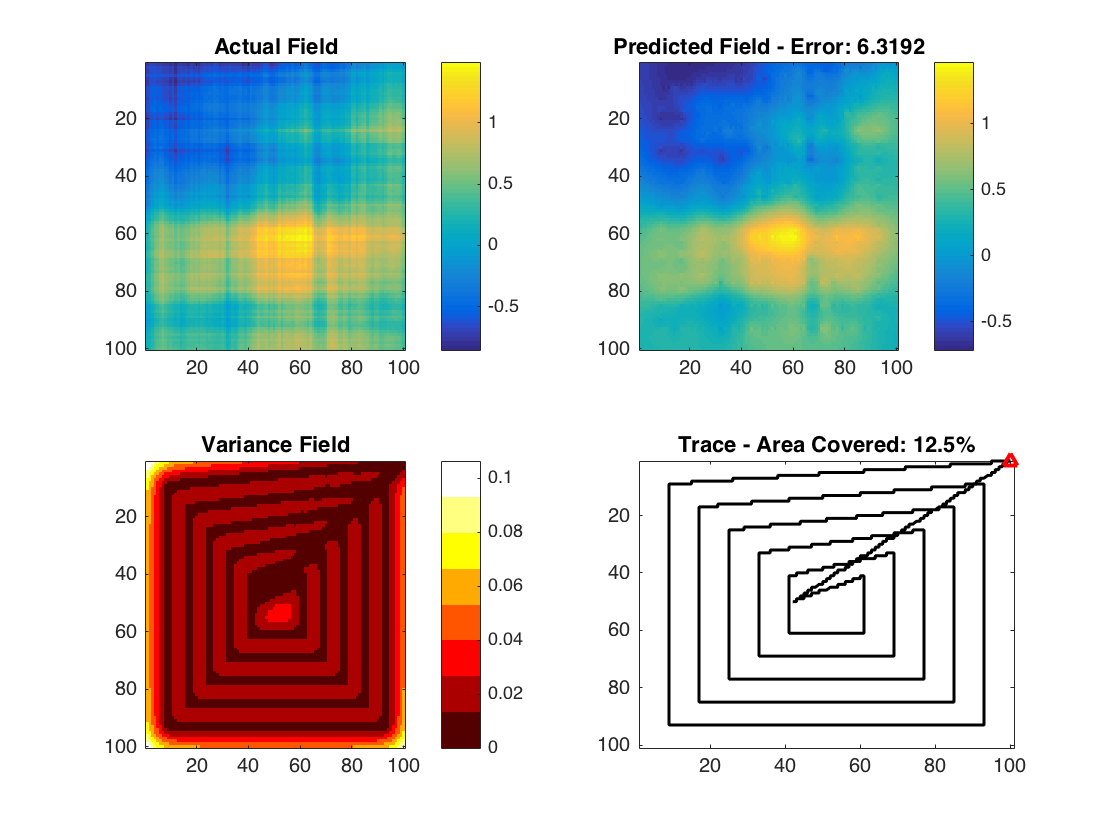
\includegraphics[width=0.9\linewidth]{figures/zigzag_4panel.png}
	\captionsetup{skip=0.20\baselineskip,size=footnotesize}
	\caption{Zig-Zag exploration method with a line spacing of $r = 8$ units. A Kriging prediction and variance calculation is computed after completing the maneuver. The actual field that is being explored is shown in the upper left. The current prediction of the actual field is shown in the upper right. The variance of the current prediction of the field is shown in the lower left. The trace of the exploration vehicle's path taken to the point of termination (in red) is shown in the lower right panel. All distance units are in meters.}
	\label{fig:zigzag4}
\end{figure}

\subsection{Prediction Error Calculation}
The quality of each path planner will be judged by its ability to explore a field in a fixed amount of time. The prediction error of each method will be used as a metric of path planning quality. The actual values of the fields scanned are known in simulation, and for each rerouting iteration, the predictions and prediction errors will be recalculated.

The prediction error function, erf$(Z,\hat{Z})$, will be the average root mean square (RMS) value for all $N$ field predictions made, point by point, on the actual field, $Z$, and the predicted field, $\hat{Z}$.

\begin{equation}
\text{erf}(Z, \hat{Z}) = \frac{1}{N}\sum_{\forall i \in Z} (Z(\vect{s}_i) - \hat{Z}(\vect{s}_i))^2
\end{equation}

\subsection{Variance Drop Calculation}
The variance of every target field over each iteration will be the average prediction variance of the field after every prediction recalculation. This criteria is introduced in Section \ref{sec:fielduncert} on field uncertainty. This metric relates prediction quality of the path planner to its predicted prediction quality. A drop in variance over iterations should signal a better prediction of the target field over that iteration, and less overall uncertainty of the target field.

\subsection{Simulation Results}
% The effectiveness of the method introduced varies based on the area of the target field being explored. For small fields, a naive zig-zag exploration may be more efficient and less computationally expensive. By modulating the dimensions of the target field, a comparison can be drawn demonstrating the effectiveness of the method versus a naive zig-zag approach.
The methods introduced will be compared to one another and the zig-zag method for the same termination condition. Each method will stop the field exploration process when the exploration vehicle traverses a fixed path length expressed in terms of the area percentage scanned, $A_{scan}$. For example, if the maximum scan percentage of a size $w \times w$ field is $p\%$, then the method will stop exploring when $A_{scan} = \frac{p}{100}w^2$ number of vesicles have been sampled. In an effort to allow the zig-zag method to cover as much of the field as possible, the spacing between each spiral bound, $r$, will be pre-calculated.

\begin{equation}
	r = \frac{A_{scan}}{2}
\end{equation}

\subsection{Simulation Result Parameters}
% n fields=3, seeds=[1,10,100]
% N=5
% N_mc=5, R_mc=10


\subsection{High Spatial Autocorrelation ($\sigma_{field} = w$) Results}
\subsubsection{Field Size of $50\times50$}
% \begin{table}[ht!]
% \centering
% 	\begin{tabular}{ |p{3cm}||p{1cm}|p{1cm}|p{1cm}|  }
% 		\hline
% 		\multicolumn{4}{|c|}{$50 \times 50$ Size Final Field Prediction Error ($\sigma_{field} = 50$)} \\
% 		\hline
% 		Coverage Limit ($A_{scan}$) & 10\% & 20\% & 30\% \\
% 		\hline
% 		Zig-Zag        & -- & -- & -- \\
% 		NHV            & -- & -- & -- \\
% 		N-NHV		   & -- & -- & -- \\
% 		MCPP  		   & -- & -- & -- \\
% 		\hline
% 	\end{tabular}
% 	\caption{Comparing field prediction errors for varying coverage limitations on a $50 \times 50$ size field ($\sigma_{field} = 50$). Random number generator seed $1$.}
%     \label{tab:50fieldprederr_1}
% \end{table}

% \begin{table}[ht!]
% \centering
% 	\begin{tabular}{ |p{3cm}||p{1cm}|p{1cm}|p{1cm}|  }
% 		\hline
% 		\multicolumn{4}{|c|}{$50 \times 50$ Size Final Field Prediction Error ($\sigma_{field} = 50$)} \\
% 		\hline
% 		Coverage Limit ($A_{scan}$) & 10\% & 20\% & 30\% \\
% 		\hline
% 		Zig-Zag        & -- & -- & -- \\
% 		NHV            & -- & -- & -- \\
% 		N-NHV		   & -- & -- & -- \\
% 		MCPP  		   & -- & -- & -- \\
% 		\hline
% 	\end{tabular}
% 	\caption{Comparing field prediction errors for varying coverage limitations on a $50 \times 50$ size field ($\sigma_{field} = 50$). Random number generator seed $2$.}
%     \label{tab:50fieldprederr_2}
% \end{table}

% \begin{table}[ht!]
% \centering
% 	\begin{tabular}{ |p{3cm}||p{1cm}|p{1cm}|p{1cm}|  }
% 		\hline
% 		\multicolumn{4}{|c|}{$50 \times 50$ Size Final Field Prediction Error ($\sigma_{field} = 50$)} \\
% 		\hline
% 		Coverage Limit ($A_{scan}$) & 10\% & 20\% & 50\% \\
% 		\hline
% 		Zig-Zag        & -- & -- & -- \\
% 		NHV            & -- & -- & -- \\
% 		N-NHV		   & -- & -- & -- \\
% 		MCPP  		   & -- & -- & -- \\
% 		\hline
% 	\end{tabular}
% 	\caption{Comparing field prediction errors for varying coverage limitations on a $50 \times 50$ size field ($\sigma_{field} = 50$). Random number generator seed $3$.}
%     \label{tab:50fieldprederr_3}
% \end{table}

\subsubsection{Field Size of $100\times100$}
% \begin{table}[ht!]
% \centering
% 	\begin{tabular}{ |p{3cm}||p{1cm}|p{1cm}|p{1cm}|  }
% 		\hline
% 		\multicolumn{4}{|c|}{$100 \times 100$ Size Final Field Variances ($\sigma_{field} = 100$)} \\
% 		\hline
% 		Coverage Limit ($A_{scan}$) & 5\% & 10\% & 20\% \\
% 		\hline
% 		Zig-Zag        & -- & -- & -- \\
% 		NHV            & -- & -- & -- \\
% 		N-NHV		   & -- & -- & -- \\
% 		MCPP  		   & -- & -- & -- \\
% 		\hline
% 	\end{tabular}
% 	\caption{Comparing field prediction errors for varying coverage limitations on a $100 \times 100$ size field ($\sigma_{field} = 100$).}
%     \label{tab:100fieldvars}
% \end{table}

\subsection{Low Spatial Autocorrelation ($\sigma_{field} = 1$) Results}
\subsubsection{Field Size of $50\times50$}
% \begin{table}[ht!]
% \centering
% 	\begin{tabular}{ |p{3cm}||p{1cm}|p{1cm}|p{1cm}|  }
% 		\hline
% 		\multicolumn{4}{|c|}{$50 \times 50$ Size Final Field Prediction Error ($\sigma_{field} = 1$)} \\
% 		\hline
% 		Coverage Limit ($A_{scan}$) & 10\% & 20\% & 50\% \\
% 		\hline
% 		Zig-Zag        & -- & -- & -- \\
% 		NHV            & -- & -- & -- \\
% 		N-NHV		   & -- & -- & -- \\
% 		MCPP  		   & -- & -- & -- \\
% 		\hline
% 	\end{tabular}
% 	\caption{Comparing field prediction errors for varying coverage limitations on a $50 \times 50$ size field ($\sigma_{field} = 1$).}
%     \label{tab:50fieldprederr}
% \end{table}

\subsubsection{Field Size of $100\times100$}
% \begin{table}[ht!]
% \centering
% 	\begin{tabular}{ |p{3cm}||p{1cm}|p{1cm}|p{1cm}|  }
% 		\hline
% 		\multicolumn{4}{|c|}{$100 \times 100$ Size Final Field Variances ($\sigma_{field} = 1$)} \\
% 		\hline
% 		Coverage Limit ($A_{scan}$) & 5\% & 10\% & 20\% \\
% 		\hline
% 		Zig-Zag        & -- & -- & -- \\
% 		NHV            & -- & -- & -- \\
% 		N-NHV		   & -- & -- & -- \\
% 		MCPP  		   & -- & -- & -- \\
% 		\hline
% 	\end{tabular}
% 	\caption{Comparing field prediction errors for varying coverage limitations on a $100 \times 100$ size field ($\sigma_{field} = 1$).}
%     \label{tab:100fieldvars}
% \end{table}
